\documentclass[12pt]{article}
\usepackage[utf8]{inputenc}
\usepackage[cm]{fullpage}
\usepackage{amssymb}
\usepackage{multicol}
\usepackage{graphicx}

\usepackage{pgffor}   % for 'for loop' usage

\usepackage{pstricks}

\newcommand{\exerc}[3]{ \vspace{5pt} {$\mathbf{#1)}$} #2 \hfill {\it #3} }
\newcommand{\exitem}[2]{ \texttt{\bf #1)} #2 \\ }

%\newcommand{\clock}[1]{
%    \psset{yunit=0.8}
%	\rput(0,0.1){
%      \foreach \n in {0,...,#1}{
%	  \translate(2,0)
%      \psline
%	    (0,0)(1,0)(1,1)(2,1)
%	  }
%	}
%    \psset{yunit=1.0}
%}

%\newcommand{\signalBlock}[1]{
%  \vspace*{20pt}
%  \hspace*{-30pt}
%  \pscustom[xunit=0.5]{
%    \rput(1,2){#1}
%  }
%}

%\newcommand{\signal}[1]{
%    \psset{yunit=0.8}
%	\rput(0,0.1){
%    \psline
%	  #1
%	  }
%    \psset{yunit=1.0}
%}

\renewcommand{\neg}[1]{ 
  \mkern 1.5mu\overline{\mkern-1.5mu#1\mkern-1.5mu}\mkern 1.5mu
}

\newenvironment{exitems}[1]{
\\
\hspace*{30pt}
\begin{minipage}{0.8\textwidth}
\begin{multicols}{#1} 
}{
\end{multicols}
\end{minipage}
}

\newenvironment{exitemss}[1]{
\\
\hspace*{30pt}
\begin{minipage}{0.8\textwidth}
#1
}{
\end{minipage}
}

\begin{document}

\pagenumbering{gobble}

\begin{center}
{\Large \bf Elementos de Lógica Digital - 2015/2}
\end{center}

\vfill

{\large \bf 1ª Lista de exercícios}

{\bf dia:} 24/09/2015

\exerc{1}{Realize as seguintes conversões entre sistemas numéricos:}{2.0 pontos}
\begin{exitems}{2}
	\exitem{a}{ $1011,010_2$ para decimal;}
	\exitem{b}{ $1011,110_2$ }
	\\
	\exitem{c}{ $19_{16}$ }
	\exitem{d}{ $4$CE$_{16}$ }
\end{exitems}

\exerc{2}{Execute as operações abaixo utilizando representação binária, utilizando a notação de complemento de 2 para números negativos.}{2.0 pontos}
\begin{exitems}{2}
	\exitem{a}{ $94-87$}
	\exitem{b}{ $41-86$}
\end{exitems}

\exerc{3}{Simplifique a expressão abaixo utilizando álgebra de Boole e monte o circuito que execute a expressão, utilizando apenas portas NOU.}{1.0 pontos}

\exerc{4}{Realize o projeto de um subtrator completo.}{2.0 pontos}

\exerc{5}{Determine a forma de onda da saída $\mathtt{Q}$ para o flip-flop JK da figura, segundo as ondas do diagrama.}{2.0 pontos}
\\
\begin{multicols}{2}
\begin{center}
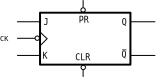
\includegraphics{fp-jk} \\ \vspace{15pt}
%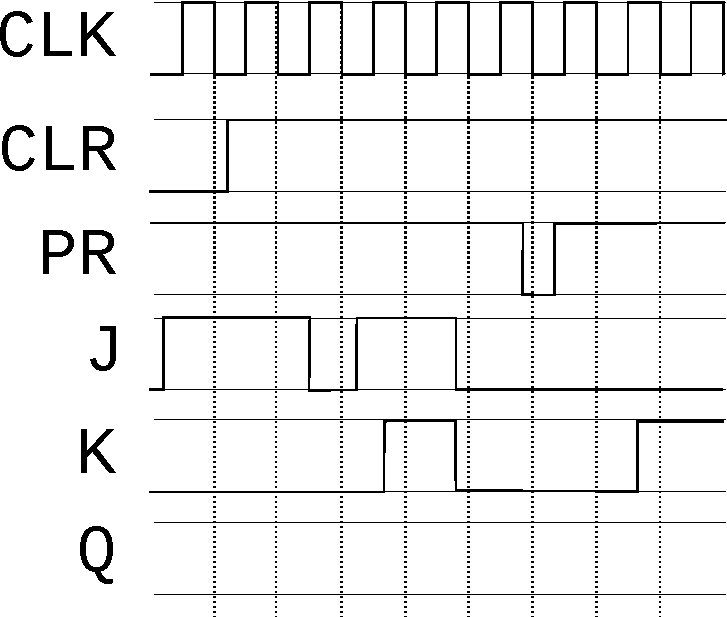
\includegraphics[scale=0.5]{sig1} \\
\end{center}
\end{multicols}

\end{document}

